\chapter{Conclusions et perspectives}
%\addcontentsline{toc}{chapter}{Conclusion}
\label{chap:conclu}

	\epigraph{«\textit{De 1580, nous passons à 1674. L'étape est longue : près d'un siècle. La nouvelle génération s'était habituée à la mansuétude, à la bénignité du Rhône, lorsque tout à coup, les eaux montèrent à une hauteur inusitée; des secours tardifs ou mal dirigés ne purent prévenir une invasion, et les chaussées succombèrent en plusieurs endroits}»}{A. Eyssette, Histoire administrative de Beaucaire depuis le XII\textsuperscript{ème} siècle jusqu'à la Révolution de 1789.}

\newpage

\paragraph{} L'objectif principal de cette thèse est de développer une méthode intégrée pour l'analyse fréquentielle des crues permettant de valoriser les enregistrements hydrométriques récents et historiques, ainsi que les recensements de crues antérieures aux relevés, avec une prise en compte complète et homogène des différentes sources d'incertitude. Même si l'utilisation de données historiques pour l'analyse fréquentielle des crues est une pratique courante, certains verrous méthodologiques restaient à débloquer pour estimer et propager l'ensemble des incertitudes. Pourtant, la prise en compte des incertitudes est particulièrement importante dans ce contexte pour plusieurs raisons. Tout d'abord, elle permet d'obtenir une estimation probabiliste du risque de crue qui est indispensable à la prise de décision éclairée. Elle permet également de comparer raisonnablement les estimations provenant de différentes méthodes pour un même site. Enfin, elle permet d'évaluer si l'ajout de données historiques, bien qu'incertaines, améliore l'estimation des quantiles extrêmes.

\paragraph{} Dans les pages suivantes, nous résumons les différentes étapes de la mise en place de cette méthode comportant un ensemble de techniques et outils, dont certains ont été développés lors de la thèse. Nous présentons également les principaux résultats de son application au cas d'étude du Rhône à Beaucaire de 1500 à 2020, qui constitue une preuve de concept permettant de tester et valider la méthode proposée, sur un cas complexe et richement documenté. Enfin, nous discutons des perspectives qui découlent de ces résultats, au-delà du cadre de la thèse et de la station de Beaucaire. 
	
	\section{Principaux résultats}
%	\addcontentsline{toc}{section}{Principaux résultats obtenus}
	
	\paragraph{} La première partie de la thèse consiste à effectuer un bilan des données de crue disponibles à Beaucaire. Cette étape ne doit pas être négligée car elle constitue les fondations de l'analyse fréquentielle. De plus, elle est tout particulièrement importante lorsque l'on s'intéresse aux incertitudes qui affectent ces données d'entrée. À Beaucaire, le précieux travail de recensement d'archives de \citet{pichard_les_1995} et \citet{pichard_hydro-climatology_2017}, ainsi que la récente étude de \citet{bard_actualisation_2018} ont permis de reconstituer une chronique continue de mesures limnimétriques débutant en 1816, ainsi que des jaugeages débutant en 1845, ce qui est remarquable. Ce premier chapitre a permis de retracer les nombreuses évolutions du chenal du Rhône à Beaucaire depuis le XIX\textsuperscript{ème} siècle, ce qui est particulièrement important afin de disposer de données objectives pour l'étude de la relation hauteur-débit (courbe de tarage) et l'estimation des incertitudes hydrométriques. Une analyse de l'évolution des temps de propagation des crues (de type océanique et inférieures à la décennale) entre Lyon et Beaucaire au cours des différentes phases d'aménagement en lit mineur a également été menée. Elle a permis de constater une diminution de ces temps de propagation, qui en 175 ans sont passés de 48 h (en valeur médiane) avant la construction des aménagements Girardon, à 16 h après la construction des aménagements CNR. Cette constatation pourrait remettre en cause la stationnarité des processus de crue de la période 1816-2020. L'étape suivante a consisté à extraire et caractériser les données de crue de la base de données HISTHRÔNE (\url{histrhone.cerege.fr}) qui recense plus de 1500 événements hydroclimatiques (crues, événements de gel du Rhône, pluies extrêmes, submersions marines) depuis le XIII\textsuperscript{ème} siècle. Une estimation de l'ordre de grandeur du débit des plus fortes crues, qui sont classées dans la base de données en différentes catégories basées sur les dommages (\og \textit{crue et inondation de gravité intermédiaire}\fg{} ou \og \textit{crue et inondation extrême}\fg{}), a été effectuée. Cette estimation se base sur le croisement des données HISTRHÔNE disponibles jusqu'en 2000 avec les hydrogrammes de la période récente (1816-2020). Cet exercice ouvre la voie à l'utilisation des crues historiques (antérieures aux mesures limnimétriques continues) pour l'analyse fréquentielle, car il permet une première approche des seuils de perception. Cependant, une évolution des enjeux en zone inondable a été mise en évidence, en lien avec la mise en place d'ouvrages de protection. Ce phénomène peut compliquer l'utilisation des seules mentions de crues, en l'absence d'estimations de débit pour chacun des événements. C'est pourquoi la piste de l'utilisation de modèles hydrauliques pour l'estimation du débit de chacune de ces crues a été explorée. Cependant, ce travail s'est heurté au manque de données, notamment pour reconstituer la bathymétrie et la rugosité du Rhône avant le XIX\textsuperscript{ème} siècle. Au regard des nombreuses incertitudes qui affectent cet exercice, de la complexité à les quantifier, et du temps limité de la thèse, nous avons décidé de ne pas poursuive la piste de la modélisation hydraulique. Néanmoins, ces travaux exploratoires ont permis de définir les contours et les limites de la modélisation du débit des crues historiques, et de dégager des pistes de simplification du modèle hydraulique pour d'éventuelles futures études.
	
	\paragraph{} Le second chapitre de la thèse a pour but d'explorer l'impact de la valorisation de données hydrométriques anciennes (et continues) sur l'analyse fréquentielle des crues. La première partie de ce travail consiste à estimer les chroniques de débit à Beaucaire de 1816 à 2020, avec une prise en compte complète des incertitudes hydrométriques. Tout d'abord, les incertitudes de mesure affectant les relevés de hauteur d'eau ont été estimées par la combinaison de diverses sources d'erreurs. Parmi ces sources, une attention particulière a été accordée à l'incertitude due à la fréquence des relevés, qui est particulièrement importante pour les mesures très anciennes. Cette incertitude a été estimée en dégradant artificiellement les données modernes, mesurées à des pas de temps très fins par des capteurs automatiques. Les dates de détarage de la relation hauteur/débit ont ensuite été estimées à l'aide de la méthode de segmentation des résidus jaugeages/courbes de tarage de \citet{darienzo_detection_2021}, dont l'intérêt principal est de pouvoir considérer l'incertitude des jaugeages dans l'estimation de ces dates. Des courbes de tarage et leurs incertitudes ont été déterminées pour chacune des périodes homogènes à l'aide de la méthode BaRatin SPD \citep{mansanarez_shift_2019}, basée sur l'interprétation physique des détarages. Cette méthode fait l'hypothèse que certains paramètres des courbes de tarage sont constants, alors que d'autres varient d'une période homogène à l'autre. Ainsi, l'information est transférée entre les périodes, ce qui permet de réduire l'incertitude des courbes de tarage en mutualisant l'information de l'ensemble des jaugeages de toutes les périodes. Les changements morphologiques identifiés au premier chapitre ont été utilisés pour la configuration de ce modèle. Ce sont ainsi 21 courbes de tarage incertaines qui ont été estimées. L'incertitude des relevés de hauteur d'eau a ensuite été propagée à travers ces courbes de tarage pour obtenir un hydrogramme incertain de 1816 à 2020. L'incertitude totale (au niveau de probabilité de 95\%) varie de 30\% au début du XIX\textsuperscript{ème} siècle, à 5\% pour les relevés les plus récents. Cette incertitude hydrométrique a ensuite été propagée jusqu'aux quantiles extrêmes estimés selon une distribution GEV via une méthode bayésienne. Ainsi, on peut déterminer la contribution de l'incertitude hydrométrique et de l'incertitude d'échantillonnage à l'incertitude totale des quantiles extrêmes. Pour la chronique complète (205 ans), l'incertitude hydrométrique est dominante pour des périodes de retour inférieures à 100 ans, alors que l'incertitude d'échantillonnage est dominante au-delà de la centennale. Les estimations GEV ont ensuite été réalisées pour des durées de chroniques variables, en sous-échantillonnant dans la chronique complète. Il apparaît que l'incertitude totale diminue significativement lorsque la durée des chroniques augmente de 20 à 100 ans. Au-delà de 100 ans, l'incertitude est très stable, ce qui suggère que le gain en termes de réduction de l'incertitude échantillonnage est compensé par la forte incertitude des données anciennes (comparativement aux données récentes). Cependant, les estimations maxpost augmentent d'environ 15\% pour des durées de chroniques supérieures à 160 ans, et ce à cause de l'inclusion des deux plus fortes crues de l'échantillon en 1840 et 1856. Ces résultats ont permis d'illustrer l'intérêt et les limites des relevés hydrométriques anciens pour la réduction des incertitudes des quantiles de crue, mais également d'identifier la part de chacune des sources d'incertitude dans cette réduction. Ils ont également permis de démontrer l'importance d'une estimation complète et homogène des incertitudes pour l'analyse fréquentielle des crues. Ces travaux ont fait l'objet d'un article scientifique soumis dans "Journal of Hydrology" et accepté sous réserve de révisions mineures.
	
	\paragraph{} Les résultats obtenus pour la chronique continue de 1816 à 2020 ont ouvert la voie à l'inclusion de données historiques antérieures aux enregistrements continus extraites de la base HISTRHÔNE. En l'absence de reconstructions du débit de chacun des événements, le nombre d'occurrences de crues supérieures à un seuil de perception a été exploité. Ce seuil de perception découle des catégories de crues de la base HISTRHÔNE : il n'a pas un sens physique uniquement déterminé par la valeur du débit, mais est également lié à la perception des dommages induits par la crue. Si l'utilisation d'un échantillon mixte (composé de données hydrométriques continues et de données de crues historiques ponctuelles) est une pratique d'analyse fréquentielle relativement commune, la propagation complète des incertitudes hydrométriques et des incertitudes d'échantillonnage est rarement abordée. De plus, le seuil de perception et la durée de la période historique durant laquelle ce dernier est actif sont dans la grande majorité des cas supposés parfaitement connus, ce qui constitue de fortes hypothèses. Le modèle proposé dans ce chapitre les considère comme des paramètres à part entière du modèle probabiliste qui sont donc à estimer. Ainsi, la méconnaissance du seuil de perception et de la durée de la période historique se reflète dans l'incertitude des résultats. Dans un premier temps, ce modèle a été appliqué à la chronique de débits continue du Rhône à Beaucaire de 1816 à 2020, qui a été artificiellement dégradée en un échantillon mixte comportant des données ponctuelles antérieures à des relevés continus. Cet exercice permet de tester le modèle sur un cas d'étude pour lequel le seuil de perception et la durée de la période historique sont parfaitement connus. Les estimations obtenues sont satisfaisantes, même si elles ne sont évidemment pas aussi précises que les estimations du chapitre précédent, qui utilisent l'entièreté de la chronique continue. Ces tests ont permis d'identifier que la seule méconnaissance du seuil de perception entraînait une incertitude bien plus grande que la seule méconnaissance de la durée de la période historique. En revanche, quand ces deux paramètres sont considérés incertains en même temps, l'incertitude des quantiles est réduite par rapport au cas où seul le seuil est incertain. Ce résultat s'explique par une corrélation entre ces deux paramètres. Ces premiers résultats démontrent également que considérer que le seuil de perception est parfaitement connu lorsque ce n'est pas le cas peut mener à une sous-estimation importante de l'incertitude des résultats. Le modèle a ensuite été appliqué aux données complètes du Rhône à Beaucaire, avec des occurrences de crues historiques pour la période 1500-1815, et la chronique de débits maximum annuels de 1816 à 2020. Les résultats présentent une incertitude réduite par rapport aux résultats de la seule chronique continue de 1816 à 2020, et ce même dans le cas où seuil de perception et durée de la période historique sont incertains (à condition d'utiliser des \textit{a priori} suffisamment informatifs). Cependant, cet exercice a permis de mettre en lumière une probable sous-estimation du nombre de dépassements du seuil de perception au cours de la période historique dans les données HISTRHÔNE. Cette potentielle non-exhaustivité apparaît alors même que la stationnarité des données a été validée. Elle pourrait provenir du fait que les catégories de la base HISTRHÔNE sont définies sur la perception des dommages par les populations ripariennes, et non sur un seuil de perception physique directement lié au dépassement d'un débit. Même si le cas d'étude de Beaucaire de 1500 à 2020 présente des limites qui semblent difficiles à surmonter, le modèle proposé dans ce chapitre ouvre la porte à une prise en compte complète et homogène des incertitudes dans le cas de l'analyse fréquentielle des crues historiques. 

\newpage
	\section{Perspectives}
%	\addcontentsline{toc}{section}{Perspectives des travaux de thèse}
	
	\begin{figure}[h!]
	\centering
		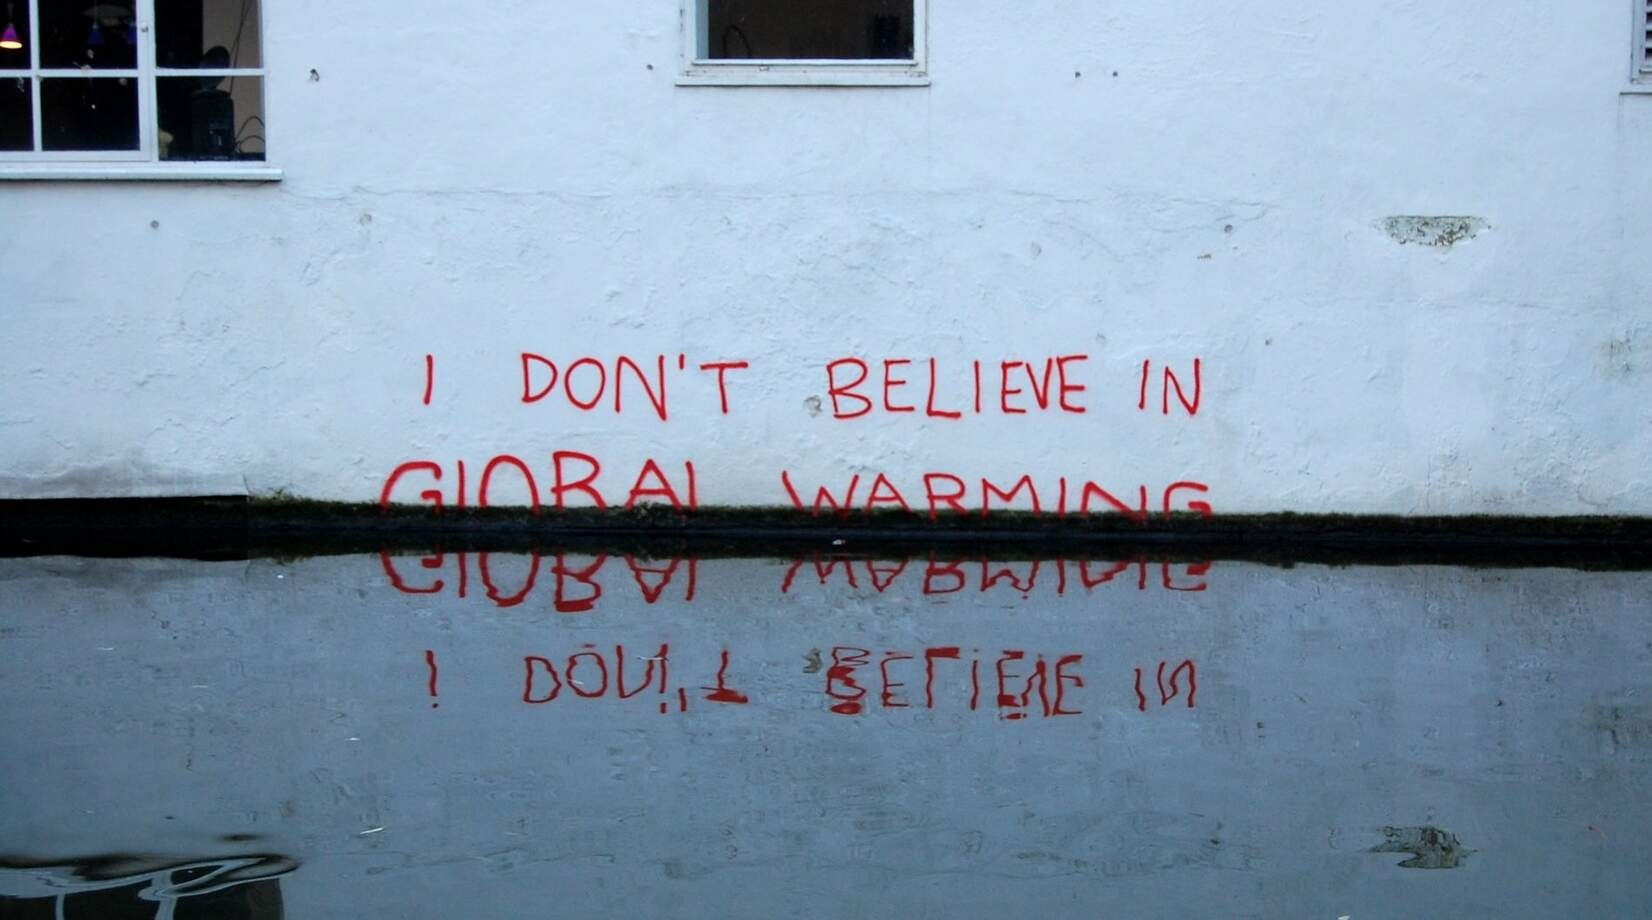
\includegraphics[width=.7\linewidth]{Chapitre5_Conclusion/Figures/gw.jpg}
        \caption{Graffiti sur un mur Londonien, attribué à l'artiste Banksy. (source : Zak Hussein)}	
		\label{fig:gw}
	\end{figure}
		
	
	\paragraph{} Les méthodes développées au cours de cette thèse comportent évidemment des limites que les pistes présentées dans cette section pourraient permettre de dépasser. 
	
	\paragraph{} Tout d'abord, l'estimation du débit des événements anciens représente un défi important que les données disponibles et la durée limitée de la thèse n'ont pas permis de relever. Pour aller plus loin à ce sujet, plusieurs pistes sont possibles. L'utilisation d'un modèle hydraulique différent pour chacune des crues étudiées semble indispensable pour s'adapter aux très nombreux scénarios possibles. Une autre grande difficulté de cet exercice est l'estimation des incertitudes associées aux débits de pointe. Elles pourraient être déterminées en réalisant des modélisations basées sur des scénarios minimum et maximum pour les paramètres et données d'entrée concernées (hauteurs de pointe atteintes, géométrie des sections, rugosité, ruptures de digues...). Au-delà de cette approche empirique, la propagation des diverses incertitudes au travers du modèle hydraulique pourrait être réalisée via l'utilisation de méthodes Monte Carlo, moyennant des temps de calculs conséquents. Pour aller plus loin, il pourrait être intéressant de réaliser des simulations en régime non-permanent afin par exemple de mieux appréhender l'impact des ruptures de digues sur le débit de pointe. En revanche, il faudrait dépasser dans certains cas le manque d'informations (spatiales et temporelles) concernant ces ruptures de digues. En restant sur un modèle hydraulique 1D, il faudrait également caler des casiers hydrauliques pour représenter les processus de stockage-déstockage en lit majeur et de laminage de la crue. Ce type de phénomène est mieux pris en compte dans les modèles 2D mais les données disponibles ne permettent pas la configuration d'un tel modèle. Une piste intéressante et à moindre coût provient de l'élaboration d'une courbe de tarage reliant les hauteurs de l'échelle reconstituée de Véran à Arles, aux débits à Beaucaire. Cette piste prometteuse a été succinctement explorée au cours de la thèse en établissant cette relation sur la période récente. Cependant, elle peut se révéler relativement incertaine dans le cas de ruptures de digues entre Beaucaire et Arles, ou dans le cas de changements importants de la répartition des débits entre le Petit-Rhône et le Grand-Rhône. Il faut cependant garder à l'esprit que, même si l'estimation du débit de chacun des événements de la base HISTRHÔNE était possible, cela ne règlerait en aucun cas les potentiels problèmes de non-exhaustivité des données. Finalement, les problématiques exposées ci-dessus devraient être explorées dans le cadre d'une collaboration forte entre hydrauliciens, géomorphologues et historiens.
	
	\paragraph{} La potentielle non-exhaustivité des données historiques identifiée au cours de la thèse est une limitation importante. Ces lacunes pourraient être comblées par l'utilisation de données complémentaires, telles que des approches de dendrochronologie \citep{ballesteros-canovas_review_2015} ou de datation des dépôts sédimentaires (\cite{dezileau_multidating_2014}; \cite{engeland_new_2020}; \cite{corella_1400-years_2021}; \cite{wilhelm_reconstructing_2022}). On peut citer notamment les études de carottes sédimentaires réalisées dans le pro-delta du Rhône par \citet{fanget_historical_2013}. Cependant, la comparaison des datations avec les occurrences de crues des deux derniers siècles ne semble pas totalement satisfaisante. De plus, ces dépôts ont probablement été fréquemment perturbés au cours de l'histoire par des remaniements sédimentaires, ce qui invite ici aussi à la prudence par rapport à la stationnarité et l'exhaustivité des données. 
	
	\paragraph{} Des pistes d'amélioration sont également envisagées sur les estimations de débit de 1816 à 2020, notamment en ce qui concerne la détection des détarages. La méthode utilisée est basée sur la segmentation des résidus jaugeages/courbes de tarage. Cependant, le faible nombre de jaugeages anciens peut conduire à une sous-estimation du nombre de détarages. Pour pallier à ce problème, il serait possible d'utiliser des méthodes de nature différente, comme l'analyse des récessions de débit (\cite{vogel_estimation_1996}; \cite{chapman_comparison_1999}; \cite{darienzo_detection_2021-1}) ou l'analyse du transport solide cumulé \citep{darienzo_detection_2021-1}. Cependant, l'application de ces méthodes est probablement limitée dans le cas de relevés limnimétriques peu fréquents. On peut également noter qu'il est sans doute possible d'améliorer l'élicitation des \textit{a priori} pour l'estimation des courbes de tarage, ce qui pourrait avoir un impact sur l'incertitude finale des hydrogrammes.	
		
		\paragraph{} Nous avons supposé que les débits maximum annuels du Rhône à Beaucaire suivent une distribution GEV. Ce choix d'une distribution pour modéliser les crues est une source d'incertitude non négligeable qui n'a pas été explorée dans cette thèse. Une manière de vérifier les résultats obtenus pourrait être de les comparer à ceux obtenus pour l'utilisation d'un échantillonnage sup-seuil et d'une distribution GPD en se basant sur les mêmes données. 		
		
	\paragraph{} Les résultats de l'analyse fréquentielle historique obtenus sont difficilement généralisables en dehors de Beaucaire. Cependant, il serait intéressant de tester le modèle d'analyse fréquentielle proposé, qui considère une incertitude sur le seuil de perception et la durée de la période historique, sur d'autres bassins versants pour lesquels des données historiques sont disponibles et dont la nature diffère de celle des données de Beaucaire (repères de crue, dendrochronologie, dépôts sédimentaires). En France, on peut notamment citer les bassins versants de l'Ardèche \citep{naulet_flood_2005} , du Gardon (\cite{neppel_flood_2010};\cite{dezileau_multidating_2014}), de l'Orbiel \citep{payrastre_usefulness_2011} ou du Rhin \citep{lang_evaluation_2022}. Il serait également possible de complexifier le modèle pour y intégrer la possibilité de considérer une incertitude sur le nombre d'occurrences de crues supérieures à un seuil, ou de considérer un seuil de perception incertain dont la magnitude varie dans le temps. Cependant, l'incertitude des estimations de tels modèles serait probablement trop importante. Il est sans doute plus utile d'investir du temps dans la recherche et la sauvegarde de données historiques dont l'exhaustivité est garantie, plutôt que de complexifier les modèles à l'infini pour les adapter à des données incomplètes. 
			
	\paragraph{} Une des perspectives les plus importantes des résultats de cette thèse serait sans doute d'utiliser la longue série de Beaucaire pour étudier la variabilité hydroclimatique sur les siècles passés, et l'impact du changement climatique. La question n'est pas simple étant donné la diversité des régimes hydrologiques que ce bassin versant agrège et le fait que l'impact du changement climatique sur les crues n'est pas homogène et reste encore très imparfaitement compris (\cite{leblois_evaluation_2002}; \cite{giuntoli_floods_2019}). La prise en compte de variables explicatives conditionnant la distribution des crues pour l'analyse fréquentielle est un sujet très largement étudié aujourd'hui, comme en témoigne la revue de \citet{salas_techniques_2018}. Il serait intéressant d'appliquer de telles méthodes à Beaucaire, par exemple via l'utilisation d'indices climatiques pouvant avoir un impact sur le bassin versant du Rhône. On peut notamment citer la NAO \citep{criado-aldeanueva_climatic_2020}, El Niño \citep{bronnimann_impact_2007}, ou les indices climatiques "cachés" proposés par \citet{renard_hidden_2021}. Enfin, au-delà de l'analyse fréquentielle des crues, la chronique du Rhône à Beaucaire pourrait être utilisée pour étudier la variabilité des crues sur le long terme, sur le modèle d'études déjà effectuées en Europe \citep{bloschl_current_2020}. Enfin, la chronique de Beaucaire a sans doute un intérêt pour l'analyse de phénomènes autres que les crues, on peut notamment penser aux étiages.
	
		\paragraph{} L'analyse régionale est un moyen fréquemment utilisé pour améliorer l'estimation des quantiles extrêmes. De plus, il est également possible de l'associer aux données historiques \citep{gaume_bayesian_2010}, ou à des méthodes d'analyse non-stationnaire \citep{han_incorporating_2022}. Cette piste a rapidement été écartée à Beaucaire car il est complexe de délimiter des régions homogènes au niveau des processus de crue pour de très grands bassins versants. Cependant, une analyse régionale à Beaucaire pourrait être effectuée en utilisant les données des stations hydrométriques du Rhône situées plus à l'amont, mais il faudrait dans ce cas prendre en compte les très fortes corrélations entre stations. On peut également mentionner la possibilité d'étudier séparément le régime des crues de chacun des grands affluents du Rhône, afin d'améliorer les estimations à Beaucaire en les conditionnant par exemple à un certain type de crue (méditerranéenne, cévenole, océanique, généralisée).
			
		\paragraph{} Les étapes de l'analyse réalisée dans ce manuscrit sont composées de plusieurs modèles, déjà existants ou développés au cours de la thèse, qui ont été assemblés pour obtenir une prise en compte complète et homogène des incertitudes. Certains de ces modèles sont aujourd'hui déjà utilisés en dehors du cadre de la recherche pour des problématiques opérationnelles. Il est donc naturel de penser à la mise au point d'une chaîne de traitement automatisée pour reproduire facilement l'analyse conduite dans cette thèse à d'autres stations hydrométriques. Ce besoin d'un traitement complet et intégral des incertitudes dans le cadre de l'analyse fréquentielle des crues peut présenter un grand intérêt pour les problématiques opérationnelles actuelles. On peut citer par exemple le besoin chez les producteurs d'énergie comme EDF ou CNR de mettre à jour régulièrement les estimations du risque de crue pour les infrastructures telles que les évacuateurs de crue des barrages ou les ouvrages de protection des centrales nucléaires. Cependant, la perspective d'une chaîne de traitement généralisable à de nombreuses stations hydrométriques semble prématurée vu les nombreuses étapes de traitement et l'expertise nécessaire à l'analyse des résultats de chacune de ces étapes (choix d'une segmentation des jaugeages, élicitation des \textit{a priori}, choix d'un modèle d'erreur sur les hauteurs d'eau, etc). De plus, les données historiques disponibles peuvent être de nature différente d'une station à l'autre et donc nécessiter un traitement différent. Une perspective plus raisonnable serait de mettre au point des outils opérationnels, généralisables, et libres d'accès pour chacune des étapes de traitement et que le fonctionnement de ces outils soit documenté et transparent. 
	
	\paragraph{} Les données hydrométriques anciennes et les informations historiques concernant les événements remarquables du passé (crues ou plus généralement risques naturels) représentent un patrimoine précieux, que ce soit pour l'analyse de la variabilité climatique long terme, ou tout simplement pour garder dans la mémoire collective l'existence de ces événements exceptionnels. Même si le Rhône peut aujourd'hui paraître très aménagé, endigué, voire même dompté, des événements dévastateurs restent possibles. La crue de décembre 2003 a fait ressurgir des peurs au sein des populations rhodaniennes, qui au fil des générations avaient oublié la gravité des crues de 1840 et 1856 malgré les avertissements de 1994 et 2002. C'est en ce sens que les initiatives de sauvetage de données similaires au projet HISTRHÔNE (à mettre à l'immense crédit de Georges Pichard) sont d'un grand intérêt, à la fois pour la science, mais également pour la sensibilisation collective aux risques naturels. En effet, le plus gros risque pour les populations ne provient peut-être pas des crues elles-mêmes, mais plutôt des mécanismes d'oubli qui interviennent au fil des générations.
	
	
